\documentclass[10pt, xcolor=x11names,compress]{beamer}
%\documentclass[t]{beamer}
\usepackage{cprotect}
\usepackage{tikz}
\usepackage{tikz-network}
\usetikzlibrary{shapes,arrows,positioning}
\usepackage{pifont}
\usepackage{tikzducks}
\usetikzlibrary{tikzmark}
\usepackage{tabulary}
\usepackage{booktabs}
\usepackage{enumitem}
\usepackage{physics}
\usepackage{float}
\usepackage{graphicx}
\usepackage{makeidx}
%\documentclass{standalone}
\usepackage{mwe}% for example pictures
\usepackage{siunitx}
\usepackage{hyperref}
\usepackage{subcaption}
\usepackage{amsmath}
\usepackage{physics}
\usepackage{siunitx}
\usepackage[dvipsnames]{xcolor}

\usecolortheme{spruce}
\useoutertheme{infolines}
\usefonttheme[onlymath]{serif}
\setbeamertemplate{headline}[default]
\setbeamertemplate{navigation symbols}{}
\mode<beamer>{\setbeamertemplate{blocks}[rounded][shadow=true]}
\setbeamercovered{transparent}
\setbeamercolor{block body}{use=structure, fg=black, bg=yellow!20}
\setbeamercolor{itemize item}{fg=black}
\setbeamercolor{itemize subitem}{fg=gray} 
\setbeamercolor{itemize subsubitem}{fg=black!20} 
% \makeatletter\setbeamertemplate{footline}
% {  
% \leavevmode%  
% \hbox{%  
% \begin{beamercolorbox}[wd=.333333\paperwidth,ht=2.25ex,dp=1ex,center]{author in head/foot}%    
% \usebeamerfont{author in head/foot}
% \insertshortauthor%~~\beamer@ifempty{\insertshortinstitute}{}
%  \end{beamercolorbox}%  
%  \begin{beamercolorbox}[wd=.333333\paperwidth,ht=2.25ex,dp=1ex,center]{institute in head/foot}%    
%  \usebeamerfont{title in head/foot}\insertinstitute  
%  \end{beamercolorbox}%  
%  \begin{beamercolorbox}[wd=.333333\paperwidth,ht=2.25ex,dp=1ex,right]{date in head/foot}%    
%  \usebeamerfont{date in head/foot}\insertshortdate{}\hspace*{2em}    
%  \insertframenumber{} / \inserttotalframenumber\hspace*{2ex}   
%  \end{beamercolorbox}}%  
%  \vskip0pt%
%  }
 \makeatother 
 \useoutertheme[footline=empty, subsection=false]{miniframes}
 \usepackage{multicol} 
 
 \author[Tamim \and Habiba \and Sithi]{
 2005095 - Tamim Hasan Saad\\
 2005096 - Habiba Rafique \\
 2005119 - Sadia afrin Sithi}
 
 \title{FORD-FULKERSON ALGORITHM}

\institute[ CSE \and BUET]{\textbf{ 
Department of CSE\\
Bangladesh University Of Engineering and Technology}}

 \date{\today} 
 \AtBeginSection{
   \frametitle{Table of Contents}
   \tableofcontents[currentsection]
}

 \begin{document}
 \frame{\titlepage}
     \begin{frame}
        \frametitle {Table of Contents}
        \tableofcontents
     \end{frame}

\section{\textbf{Scenarios} }
\begin{frame}{Scenarios}
\begin {center} 
   \begin {minipage} {0.7\textwidth}
     \begin{block}{Some real life scenarios!!}
         $\rightarrow$ Network Traffic Optimization\\
         $\rightarrow$ Water Distribution Systems\\
         $\rightarrow$ Electric Power Grids\\
         $\rightarrow$ Network reliability\\
         $\rightarrow$ Airline scheduling\\
         $\rightarrow$ Baseball elimination\\
         $\rightarrow$ Distributed computing\\
         and many many more . . .
    \end{block}
  \end{minipage}
\end{center}
\end{frame}
    
\begin{frame}{An Example}
    %\newpage
    \begin{figure}
    \centering        
        \includegraphics[height=6.5cm, width=10cm ]{image1.jpg}
        \label{fig:enter-label}
    \end{figure}   
\end{frame}

\section{\textbf{Introduction}}
\begin{frame}{Introduction}
\begin{center}
   \begin {minipage} {0.8\textwidth}
    \begin{block}{Network FLow}
     A Network is a directed graph {\color{blue}\textbf{G}}\\
     Edges represent pipes that carry flow\\
     Each edge ${\color{blue}{<}}$ ${\color{blue}{\textbf{u,v}}}$ ${\color{blue}{>}}$ has a maximum capacity  ${\color{blue}{c{<}}}$ ${\color{blue}{\textbf {u,v}}}$ ${\color{blue}{>}}$\\
     A source node {\color{blue}\textbf{s}} in which flow arrives\\
     A sink node {\color{blue}\textbf{t}} out which flow leaves
     \end{block}
     \begin{block}{Value of a Flow}
     $|f| = \sum_{v \in V}(s,v) = \sum_{v \in V}(v,t)$\\
     This is the total flow leaving s = the total flow arriving in t. 
     \end{block} 
     \end{minipage}
\end{center}
\end{frame}

\begin{frame}{Introduction}  
    \begin{block}{Definition}
    The Ford-Fulkerson algorithm efficiently solves the maximum flow problem in a network by determining the maximum amount of flow from a source to a sink, respecting edge capacity constraints.
    \end{block}  
\end{frame}

\begin{frame}{History}
    \begin{block}{Inventors}
        This algorithm was discovered in 1956 by Ford and Fulkerson.
    \end{block}
    \begin{table}[h]
         \centering
         \begin{tabular}{c c} 
              \includegraphics[scale=0.65]{images/ford.png} & \includegraphics[scale=0.70]{images/Delbert_Ray_Fulkerson.png}\\
              \textbf{\textit{L.R.Ford,Jr.}} & \textbf{\textit{Delbert Ray Fulkerson}}
          \end{tabular}
    \end{table}
\end{frame}

\section{\textbf{Problem Description}}
\begin{frame}[t]{The Problem}
\begin{block}{}
Use a graph to model material that flows through conduits.
Each edge represents one conduit, and has a capacity, which is an upper bound on the flow rate = units/time.
Can think of edges as pipes of different sizes. 
Want to compute max rate that we can ship material from a designated source to a designated sink.
\end{block}


\begin{figure}
    \centering
    \includegraphics[height=4cm, width=9cm ]{image2.jpg}
    % \caption{Caption}
    \label{fig:enter-label}
\end{figure}
\end{frame}

\begin{frame}[t]{The Problem}
\begin {center} 
\begin {minipage} {0.7\textwidth}
\begin{block}{}
        \begin{itemize}
        \item [$\blacksquare$]Each edge (u,v) has a nonnegative capacity c(u,v). 
        \item [$\blacksquare$] If (u,v) is not in E, assume c(u,v)=0.
        \item [$\blacksquare$]We have a source s, and a sink t. 
        \item [$\blacksquare$]Assume that every vertex v in V is on some path from s to t. 
        \item [$\blacksquare$]c(s,v1)=16; c(v1,s)=0; c(v2,v3)=0
    \end{itemize}
\end{block}
\end{minipage}
\end{center}


\begin{figure}
    \centering
    \includegraphics[height=4cm, width=9cm ]{image2.jpg}
    % \caption{Caption}
    \label{fig:enter-label}
\end{figure}
\end{frame}

\section{\textbf{Properties}}
\subsection{\textbf{Residual Graph}}
\begin{frame}[t]{Residual Network}
   \begin {center} 
   \begin {minipage} {0.8\textwidth} 
     \begin{block}{Residual Graph}
         $\rightarrow$ Original edge: e = (u, v) \in E.\\     
         &\quad \quad Flow f(e), capacity c(e).\\ 
         $\rightarrow$ Create two residual edges\\
         &\quad \quad\textbf{Forward edge}\\
         &\quad \quad \quad e = (u, v) with capacity c(e) - f(e)\\
         &\quad \quad \textbf{Backward/reverse edge} \\
         &\quad \quad \quad e’ = (v, u) with capacity f(e)\\
         $\rightarrow$ Residual graph: $G_f$ = (V, $E_f$ )\\
         where,\\
         $E_f$ = edges with positive residual capacity\\
         $E_f$ = $\{e : f(e) < c(e)\} \cup \{e’ : f(e) > 0\}$
     \end{block}
\end{minipage}
\end{center}   
\end{frame}

\begin{frame}{Residual Network}
\begin{center}
    
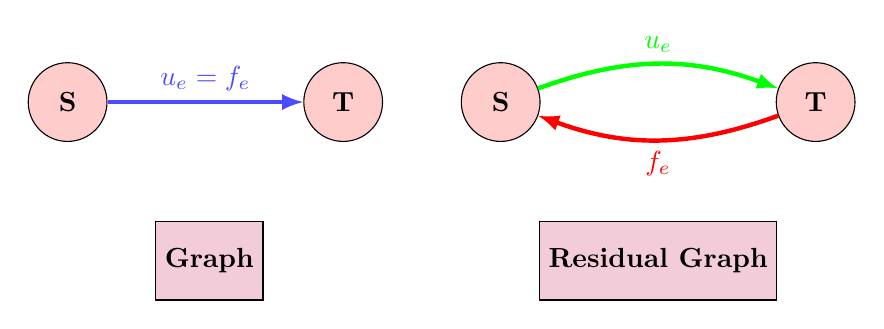
\begin{tikzpicture}

\node[draw, circle, fill=red!20, text=black, font=\bfseries, minimum size=1cm
] (IS) {S};
\node[draw, circle, fill=red!20, text=black, font=\bfseries, minimum size=1 cm, xshift=3.5 cm] (IT) {T};
\node[draw, circle, fill=red!20, text=black, font=\bfseries, minimum size=1cm, xshift=5.5 cm] (FS) {S};
\node[draw, circle, fill=red!20, text=black, font=\bfseries, minimum size=1cm, xshift=9.5 cm] (FT) {T};

\node[draw, fill=purple!20, text=black, font=\bfseries, minimum height=1cm, below=1cm of IS, xshift=1.8cm] (Graph) {Graph};

\node[draw, fill=purple!20, text=black, font=\bfseries, minimum height=1cm, below=1cm of FS, xshift=2cm] (Residual Graph) {\textbf{Residual Graph}};



    \draw[->, blue!70, ultra thick, >=latex] (IS) -- node[above, sloped, 
    font=\bfseries\color{blue}] {\textbf{$u_e = f_e$}} (IT);
    \draw[->, green, ultra thick, bend left=20, >=latex] (FS) to node[above, font=\bfseries\color{green}] {$u_e$} (FT);
    \draw[->, red, ultra thick, bend left=20, >=latex] (FT) to node[below, font=\bfseries\color{red}] {$f_e$} (FS);

        
\end{tikzpicture}
\end{center}
\end{frame}

\begin{frame}{}
    \large \textbf{Why do we need \textbf{residual networks}?}
    \begin{center}
    \begin{block}{}
        \begin{itemize}
            \item[$\blacksquare$] Allow us to reverse flow if necessary
            \item[$\blacksquare$] If we take a bad path then it will be helpful
            \item[$\blacksquare$] The bad path will overlap with too many paths..... 
        \end{itemize} 
    \end{block}
    \end{center}
\end{frame}



\subsection{\textbf{Augmenting Path}}
\begin{frame}{Augmenting Path}
   \begin {center} 
   \begin {minipage} {0.9\textwidth}
    \begin{block}{Definition}
        An augmenting path P is a simple path from s to t on the residual network. 
    \end{block}
    \begin{block}{Idea}
       Increase flow on forward edges\\
       Decrease flow on backward edges     
    \end{block}
    
    \begin{block}{Bottleneck capacity}
        let bottleneck(P, f) be the minimum residual
        capacity (i.e., capacity in $G_f$) of any edge in P
        \end{block}
    \end{minipage}
\end{center}    
        \centering
    $C_f(P) = \min \left\{ (u,v) : (u,v) \text{ is on } P \right\}$

\end{frame}


\begin{frame}{Augmenting Path}
\begin{center}
    
\begin{tikzpicture}
\node[draw, circle, fill=red!60, text=black, font=\bfseries, minimum size=0.5cm] (ZS) {S};
\node[draw, circle, fill=red!60, text=black, font=\bfseries, minimum size=0.5 cm, xshift=2.2 cm,yshift=1.2cm] (ZA) {A};
\node[draw, circle, fill=red!60, text=black, font=\bfseries, minimum size=0.5cm, xshift=5.8 cm,yshift=1.2cm] (ZB) {B};
\node[draw, circle, fill=red!30, text=black, font=\bfseries, minimum size=0.5cm, xshift=2.2 cm,yshift=-1.2cm] (ZC) {C};
\node[draw, circle, fill=red!30, text=black, font=\bfseries, minimum size=0.5cm, xshift=5.8 cm,yshift=-1.2cm] (ZD) {D};
\node[draw, circle, fill=red!60, text=black, font=\bfseries, minimum size=0.5 cm, xshift=8 cm] (ZF) {F};
% \node[draw, fill=green!20, text=black, font=\bfseries, minimum height=1cm, below=1cm of ZC, xshift=1.8cm] (ZLABEL) {Augmenting path which is a simple path from the source to the sink\\ Here is a augmenting path: S \rightarrow A \rightarrow B \rightarrow F};

\node[draw, fill=purple!10, text=black, font=\bfseries, minimum height=1cm, below=1cm of ZC, xshift=1.8cm, text width=10cm, align=center] (ZLABEL) {Augmenting path which is a simple path from the source to the sink.\\Here is an augmenting path:\\ \textbf{ S $\rightarrow$ A $\rightarrow$ B $\rightarrow$ F}\\ Bottleneck capacity is the minimum capacity of augmenting path.Here Bottleneck capacity is \textbf{8} which is the minimum of the three edges in augmenting path };


    \draw[->, blue, ultra thick, >=latex] (ZS) -- node[above, sloped, font=\bfseries\color{blue}] {$\textbf{8/9}$} (ZA);
    \draw[->, thin >=latex] (ZS) -- node[below, sloped, font=\bfseries\color{blue}] {} (ZC);

    \draw[->, blue, ultra thick, >=latex] (ZA) -- node[above, sloped, font=\bfseries\color{blue}] {$\textbf{8/10}$} (ZB);
    \draw[->, thin, >=latex] (ZA) -- node[  font=\bfseries\color{blue}] {} (ZC);
    \draw[->, blue, ultra thick, >=latex] (ZB) -- node[above, sloped,font=\bfseries\color{blue}] {$\textbf{8/8}$} (ZF);
    \draw[->, thin, >=latex] (ZC) -- node[ font=\bfseries\color{blue}] {} (ZB);
    \draw[->, thin, >=latex] (ZC) -- node[ font=\bfseries\color{blue}] {} (ZD);
    \draw[->, thin, >=latex] (ZD) -- node[ font=\bfseries\color{blue}] {} (ZB);
    \draw[->, thin, >=latex] (ZD) -- node[ font=\bfseries\color{blue}] {} (ZF);

            
            
  
\end{tikzpicture}
\end{center}

\end{frame}


\begin{frame}{Augmenting Path}
\textbf{Use path P in $G_f$ to to update flow f}
\begin {center} 
\begin {minipage} {0.8\textwidth}
\begin{block}
\centering
\begin{align*}
&\text{Augment}(f, P) \{  \quad  \text{\textcolor{blue}{// edge on P with least residual capacity}}\\
&\quad b = \text{bottleneck}(P, f) \\
&\quad \text{foreach } e = (u,v) \in P \{ \\
&\quad\quad \text{if } e \text{ is a forward edge} \\
&\quad\quad\quad f(e) = f(e) + b \quad  \text{\textcolor{blue}{//forward edge: increase flow}}\\
&\quad\quad \text{else} \\
&\quad\quad\quad \text{let } e' = (v, u) \\
&\quad\quad\quad f(e') = f(e') - b \quad  \text{\textcolor{blue}{//backward edge: decrease flow}} \\
&\quad \} \\
&\quad \text{return } f \\
&\}
\end{align*}
\end{block}
\end{minipage}
\end{center}
\end{frame}



\subsection{\textbf{Ford-Fulkerson}}
\begin{frame}{Ford-Fulkerson Method}
\begin{center}
    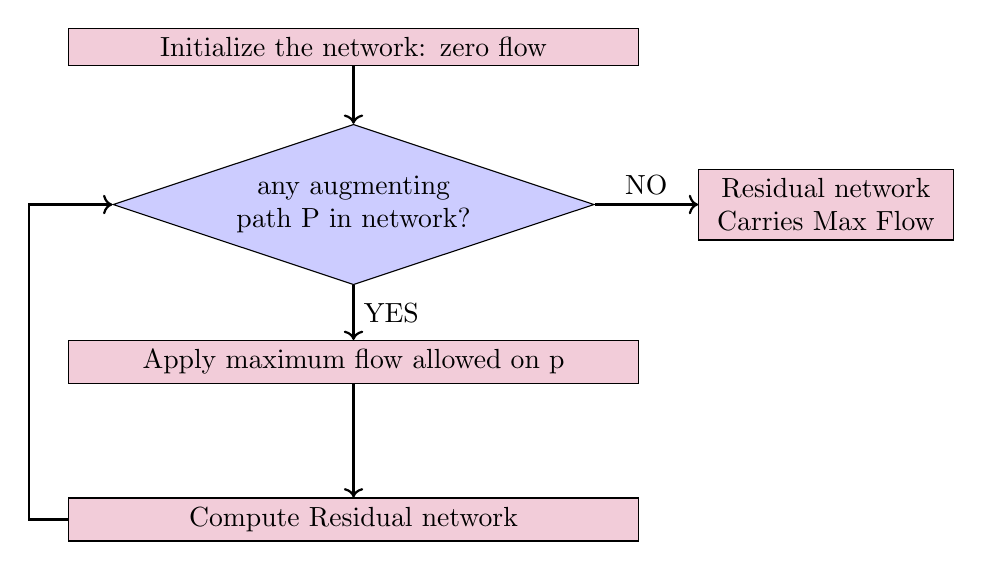
\begin{tikzpicture}
       %Defining nodes
       \node[draw, rectangle, draw=black, fill=purple!20, text width=7cm, text centered](Initialize){Initialize the network: zero flow};
       
       \node[draw, diamond, draw=black, fill=blue!20, text width=3cm, text centered, below of=Initialize, yshift=-1cm, aspect=3] (Decision) {any augmenting path P in network?}; %aspect use for make that chapta
       
       \node[draw, rectangle, draw=black, fill=purple!20, text width=7cm, text centered, below of=Decision, yshift=-1cm,](Yes){Apply maximum flow allowed on p};
       
       \node[draw, rectangle, draw=black, fill=purple!20, text width=3cm, text centered, right of=Decision, xshift=5cm,](No){Residual network Carries Max Flow};
       
       \node[draw, rectangle, draw=black, fill=purple!20, text width=7cm, text centered, below of=Yes, yshift=-1cm,](Compute){Compute Residual network};

       %Drawing Diagram
       \draw[black, thick, ->] (Initialize.south) -- (Decision.north);
       \draw[black, thick, ->] (Decision.south) -- node[pos=0.5,right] {YES} (Yes.north);
       \draw[black, thick, ->] (Decision.east) -- node[pos=0.5, above] {NO} (No.west);
       \draw[black, thick, ->] (Yes.south) -- (Compute.north);
       \draw[black, thick, ->] (Compute.west) -- ++(-0.5,0) |- (Decision.west);
       %\draw[black, thick, ->] (Decision.west) -| (Attend.north);
    \end{tikzpicture}
 \end{center} 
\end{frame}

\begin{frame}{Ford-Fulkerson Algorithm}
\textbf{Repeat: find an augmenting path, and augment!}
\begin {center} 
\begin {minipage} {0.8\textwidth}
\begin{block}
\centering
\begin{align*}
&\text{Ford-Fulkerson}(G, s, t) \{\\ 
&\quad \text{foreach e} \in E \quad f(e) = 0 \text{\textcolor{blue}{\quad //initially, no flow}}\\
&\quad G_{\textit{f}} = \text{copy of G} \text{\textcolor{blue}{\quad //residual graph = original graph}}\\ 
&\quad \text{while (there exists an s-t path P in } G_{\text{f}})\{\\
&\quad \quad f =\text{ Augment}(f, P) \text{\textcolor{blue}{\quad //change the flow}}\\ 
&\quad \quad \text{update } G_{\text{f}} \text{\textcolor{blue}{\quad //build a new residual graph}}\\
&\quad \} \\
&\quad \text{return} f\\
&\}
\end{align*}

\end{block}
\end{minipage}
\end{center}
\end{frame}



%%%%%%%%%%-------- dont touch here, -----------%%%%%%%%%%%%%

\section{\textbf{Example}}
\begin{frame}[m]{An Example}
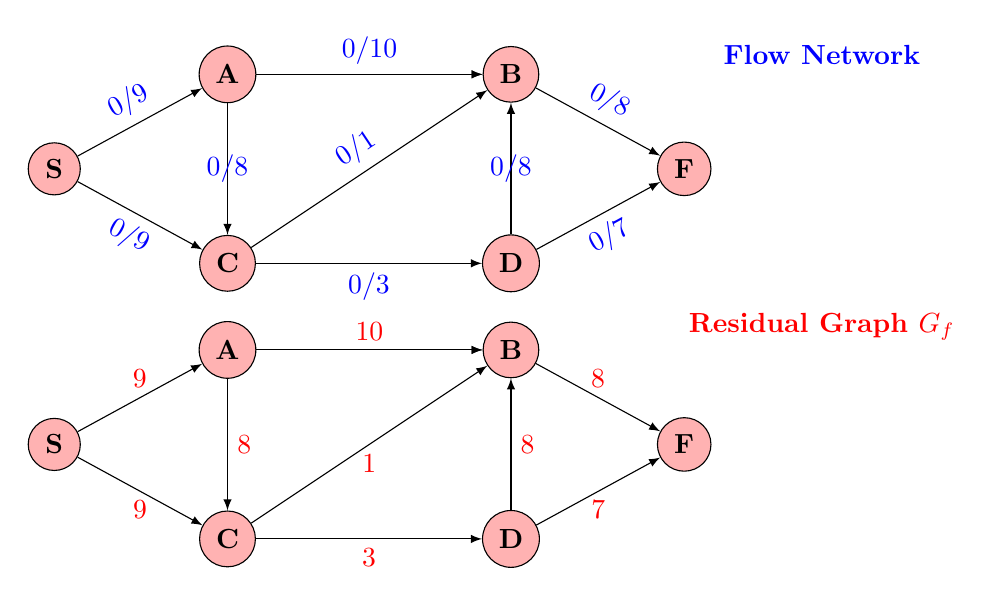
\begin{tikzpicture}
\node[draw, circle, fill=red!30, text=black, font=\bfseries, minimum size=0.5cm] (S) {S};
\node[draw, circle, fill=red!30, text=black, font=\bfseries, minimum size=0.5 cm, xshift=2.2 cm,yshift=1.2cm] (A) {A};
\node[draw, circle, fill=red!30, text=black, font=\bfseries, minimum size=0.5cm, xshift=5.8 cm,yshift=1.2cm] (B) {B};
\node[draw, circle, fill=red!30, text=black, font=\bfseries, minimum size=0.5cm, xshift=2.2 cm,yshift=-1.2cm] (C) {C};
\node[draw, circle, fill=red!30, text=black, font=\bfseries, minimum size=0.5cm, xshift=5.8 cm,yshift=-1.2cm] (D) {D};
\node[draw, circle, fill=red!30, text=black, font=\bfseries, minimum size=0.5 cm, xshift=8 cm] (F) {F};
%============
\node[draw, circle, fill=red!30, text=black, font=\bfseries, minimum size=0.5cm, below of=S, yshift=-2.5cm] (RS) {S};
\node[draw, circle, fill=red!30, text=black, font=\bfseries, minimum size=0.5 cm,below of=A, yshift=-2.5cm] (RA) {A};
\node[draw, circle, fill=red!30, text=black, font=\bfseries, minimum size=0.5cm, below of=B, yshift=-2.5cm] (RB) {B};
\node[draw, circle, fill=red!30, text=black, font=\bfseries, minimum size=0.5cm, below of=C, yshift=-2.5cm] (RC) {C};
\node[draw, circle, fill=red!30, text=black, font=\bfseries, minimum size=0.5cm, below of=D, yshift=-2.5cm] (RD) {D};
\node[draw, circle, fill=red!30, text=black, font=\bfseries, minimum size=0.5 cm,below of=F, yshift=-2.5cm] (RF) {F};
%==========

            \draw[->, thin, >=latex] (S) -- node[above, sloped, font=\bfseries\color{blue}] {$0/9$} (A);
            \draw[->, thin, >=latex] (S) -- node[below, sloped, font=\bfseries\color{blue}] {$0/9$} (C);
            \draw[->, thin, >=latex] (A) -- node[pos = 2.5,above, sloped, font=\bfseries\color{blue}] {Flow Network} (B);
            \draw[->, thin, >=latex] (A) -- node[above, sloped, font=\bfseries\color{blue}] {$0/10$} (B);
            \draw[->, thin, >=latex] (A) -- node[
            font=\bfseries\color{blue}] {$0/8$} (C);
            \draw[->, thin, >=latex] (B) -- node[above, sloped, font=\bfseries\color{blue}] {$0/8$} (F);
            \draw[->, thin, >=latex] (C) -- node[above, sloped, font=\bfseries\color{blue}] {$0/1$} (B);
            \draw[->, thin, >=latex] (C) -- node[below, sloped, font=\bfseries\color{blue}] {$0/3$} (D);
            \draw[->, thin, >=latex] (D) -- node[
            font=\bfseries\color{blue}] {$0/8$} (B);
            \draw[->, thin, >=latex] (D) -- node[below, sloped, font=\bfseries\color{blue}] {$0/7$} (F);
            
            % \draw[->, bend left=11]  (B) to (D);
            % \draw[->, bend left=11]  (D) to (B);

            \draw[->, thin, >=latex] (RS) -- node[above, font=\bfseries\color{red}] {$9$} (RA);
            \draw[->, thin, >=latex] (RS) -- node[below, font=\bfseries\color{red}] {$9$} (RC);
            \draw[->, thin, >=latex] (RA) -- node[pos = 2.5,above, font=\bfseries\color{red}] {Residual Graph $G_f$} (RB);
            \draw[->, thin, >=latex] (RA) -- node[above, font=\bfseries\color{red}] {$10$} (RB);
            \draw[->, thin, >=latex] (RA) -- node[right,
            font=\bfseries\color{red}] {$8$} (RC);
            \draw[->, thin, >=latex] (RB) -- node[above,  font=\bfseries\color{red}] {$8$} (RF);
            \draw[->, thin, >=latex] (RC) -- node[below, font=\bfseries\color{red}] {$1$} (RB);
            \draw[->, thin, >=latex] (RC) -- node[below, font=\bfseries\color{red}] {$3$} (RD);
            \draw[->, thin, >=latex] (RD) -- node[right,
            font=\bfseries\color{red}] {$8$} (RB);
            \draw[->, thin, >=latex] (RD) -- node[below, font=\bfseries\color{red}] {$7$} (RF);
  
\end{tikzpicture}

\end{frame}
%===========2========================
\begin{frame}{An Example}

\begin{tikzpicture}
\node[draw, circle, fill=red!30, text=black, font=\bfseries, minimum size=0.5cm] (S) {S};
\node[draw, circle, fill=red!30, text=black, font=\bfseries, minimum size=0.5 cm, xshift=2.2 cm,yshift=1.2cm] (A) {A};
\node[draw, circle, fill=red!30, text=black, font=\bfseries, minimum size=0.5cm, xshift=5.8 cm,yshift=1.2cm] (B) {B};
\node[draw, circle, fill=red!30, text=black, font=\bfseries, minimum size=0.5cm, xshift=2.2 cm,yshift=-1.2cm] (C) {C};
\node[draw, circle, fill=red!30, text=black, font=\bfseries, minimum size=0.5cm, xshift=5.8 cm,yshift=-1.2cm] (D) {D};
\node[draw, circle, fill=red!30, text=black, font=\bfseries, minimum size=0.5 cm, xshift=8 cm] (F) {F};
%============
\node[draw, circle, fill=red!30, text=black, font=\bfseries, minimum size=0.5cm, below of=S, yshift=-2.5cm] (RS) {S};
\node[draw, circle, fill=red!30, text=black, font=\bfseries, minimum size=0.5 cm,below of=A, yshift=-2.5cm] (RA) {A};
\node[draw, circle, fill=red!30, text=black, font=\bfseries, minimum size=0.5cm, below of=B, yshift=-2.5cm] (RB) {B};
\node[draw, circle, fill=red!30, text=black, font=\bfseries, minimum size=0.5cm, below of=C, yshift=-2.5cm] (RC) {C};
\node[draw, circle, fill=red!30, text=black, font=\bfseries, minimum size=0.5cm, below of=D, yshift=-2.5cm] (RD) {D};
\node[draw, circle, fill=red!30, text=black, font=\bfseries, minimum size=0.5 cm,below of=F, yshift=-2.5cm] (RF) {F};
%==========

            \draw[->, blue, ultra thick, >=latex] (S) -- node[above, sloped, font=\bfseries\color{blue}] {$\textbf{8/9}$} (A);
            \draw[->, thin >=latex] (S) -- node[below, sloped, font=\bfseries\color{blue}] {$0/9$} (C);
            \draw[->, thin, >=latex] (A) -- node[pos = 2.5,above, sloped, font=\bfseries\color{blue}] {Flow Network} (B);
            \draw[->, blue, ultra thick, >=latex] (A) -- node[above, sloped, font=\bfseries\color{blue}] {$\textbf{8/10}$} (B);
            \draw[->, thin, >=latex] (A) -- node[
            font=\bfseries\color{blue}] {$0/8$} (C);
            \draw[->, blue, ultra thick, >=latex] (B) -- node[above, sloped, font=\bfseries\color{blue}] {$\textbf{8/8}$} (F);
            \draw[->, thin, >=latex] (C) -- node[above, sloped, font=\bfseries\color{blue}] {$0/1$} (B);
            \draw[->, thin, >=latex] (C) -- node[below, sloped, font=\bfseries\color{blue}] {$0/3$} (D);
            \draw[->, thin, >=latex] (D) -- node[
            font=\bfseries\color{blue}] {$0/8$} (B);
            \draw[->, thin, >=latex] (D) -- node[below, sloped, font=\bfseries\color{blue}] {$0/7$} (F);
            
            % \draw[->, bend left=11]  (B) to (D);
            % \draw[->, bend left=11]  (D) to (B);

            \draw[->, thin, >=latex] (RS) -- node[above, font=\bfseries\color{red}] {$9$} (RA);
            \draw[->, thin, >=latex] (RS) -- node[below, font=\bfseries\color{red}] {$9$} (RC);
            \draw[->, thin, >=latex] (RA) -- node[pos = 2.5,above, font=\bfseries\color{red}] {Residual Graph $G_f$} (RB);
            \draw[->, thin, >=latex] (RA) -- node[above, font=\bfseries\color{red}] {$10$} (RB);
            \draw[->, thin, >=latex] (RA) -- node[right,
            font=\bfseries\color{red}] {$8$} (RC);
            \draw[->, thin, >=latex] (RB) -- node[above,  font=\bfseries\color{red}] {$8$} (RF);
            \draw[->, thin, >=latex] (RB) -- node[pos = 2.5, above, font=\bfseries\color{black}] {\parbox{3cm}{\centering Start: \\ F(u,v) = 0 for all edges \\ $F_m = 0$}} (RF);
            \draw[->, thin, >=latex] (RC) -- node[below, font=\bfseries\color{red}] {$1$} (RB);
            \draw[->, thin, >=latex] (RC) -- node[below, font=\bfseries\color{red}] {$3$} (RD);
            \draw[->, thin, >=latex] (RD) -- node[right,
            font=\bfseries\color{red}] {$8$} (RB);
            \draw[->, thin, >=latex] (RD) -- node[below, font=\bfseries\color{red}] {$7$} (RF);
  
\end{tikzpicture}
    
\end{frame}
%==================3============
\begin{frame}{An Example}
% \begin{columns}
%     \begin{column}{0.7\linewidth}

\begin{tikzpicture}
\node[draw, circle, fill=red!30, text=black, font=\bfseries, minimum size=0.5cm] (S) {S};
\node[draw, circle, fill=red!30, text=black, font=\bfseries, minimum size=0.5 cm, xshift=2.2 cm,yshift=1.2cm] (A) {A};
\node[draw, circle, fill=red!30, text=black, font=\bfseries, minimum size=0.5cm, xshift=5.8 cm,yshift=1.2cm] (B) {B};
\node[draw, circle, fill=red!30, text=black, font=\bfseries, minimum size=0.5cm, xshift=2.2 cm,yshift=-1.2cm] (C) {C};
\node[draw, circle, fill=red!30, text=black, font=\bfseries, minimum size=0.5cm, xshift=5.8 cm,yshift=-1.2cm] (D) {D};
\node[draw, circle, fill=red!30, text=black, font=\bfseries, minimum size=0.5 cm, xshift=8 cm] (F) {F};
%============
\node[draw, circle, fill=red!30, text=black, font=\bfseries, minimum size=0.5cm, below of=S, yshift=-2.5cm] (RS) {S};
\node[draw, circle, fill=red!30, text=black, font=\bfseries, minimum size=0.5 cm,below of=A, yshift=-2.5cm] (RA) {A};
\node[draw, circle, fill=red!30, text=black, font=\bfseries, minimum size=0.5cm, below of=B, yshift=-2.5cm] (RB) {B};
\node[draw, circle, fill=red!30, text=black, font=\bfseries, minimum size=0.5cm, below of=C, yshift=-2.5cm] (RC) {C};
\node[draw, circle, fill=red!30, text=black, font=\bfseries, minimum size=0.5cm, below of=D, yshift=-2.5cm] (RD) {D};
\node[draw, circle, fill=red!30, text=black, font=\bfseries, minimum size=0.5 cm,below of=F, yshift=-2.5cm] (RF) {F};
%==========

            \draw[->, blue, ultra thick, >=latex] (S) -- node[above, sloped, font=\bfseries\color{blue}] {$\textbf{8/9}$} (A);
            \draw[->, thin >=latex] (S) -- node[below, sloped, font=\bfseries\color{blue}] {$0/9$} (C);
            \draw[->, thin, >=latex] (A) -- node[pos = 2.5,above, sloped, font=\bfseries\color{blue}] {Flow Network} (B);
            \draw[->, blue, ultra thick, >=latex] (A) -- node[above, sloped, font=\bfseries\color{blue}] {$\textbf{8/10}$} (B);
            \draw[->, thin, >=latex] (A) -- node[
            font=\bfseries\color{blue}] {$0/8$} (C);
            \draw[->, thin, >=latex] (B) -- node[pos = 2.5, above, font=\bfseries\color{black}] {\parbox{3cm}{$F_m = 0 + 8 = 8$ \\ Augmenting Path: $S \rightarrow A \rightarrow B \rightarrow F$}} (F);
            \draw[->, blue, ultra thick, >=latex] (B) -- node[above, sloped, font=\bfseries\color{blue}] {$\textbf{8/8}$} (F);
            \draw[->, thin, >=latex] (C) -- node[above, sloped, font=\bfseries\color{blue}] {$0/1$} (B);
            \draw[->, thin, >=latex] (C) -- node[below, sloped, font=\bfseries\color{blue}] {$0/3$} (D);
            \draw[->, thin, >=latex] (D) -- node[
            font=\bfseries\color{blue}] {$0/8$} (B);
            \draw[->, thin, >=latex] (D) -- node[below, sloped, font=\bfseries\color{blue}] {$0/7$} (F);
            
            % \draw[->, bend left=11]  (B) to (D);
            % \draw[->, bend left=11]  (D) to (B);


            \draw[->, thin, >=latex] (RS) -- node[below, font=\bfseries\color{red}] {$9$} (RC);
  
            \draw[->, thin, >=latex] (RA) -- node[right,
            font=\bfseries\color{red}] {$8$} (RC);

            \draw[->, thin, >=latex] (RC) -- node[below, font=\bfseries\color{red}] {$1$} (RB);
            \draw[->, thin, >=latex] (RC) -- node[below, font=\bfseries\color{red}] {$3$} (RD);
            \draw[->, thin, >=latex] (RD) -- node[right,
            font=\bfseries\color{red}] {$8$} (RB);
            \draw[->, thin, >=latex] (RD) -- node[below, font=\bfseries\color{red}] {$7$} (RF);


             \draw[->, red, ultra thick, bend left=11, >=latex] (RA) to node[below, font=\bfseries\color{red}] {$\textbf{8}$} (RS);
             \draw[->, green, ultra thick, bend left=11, >=latex] (RS) to node[above, font=\bfseries\color{green}] {$\textbf{1}$} (RA);

             \draw[->, red, ultra thick, bend left=11, >=latex] (RB) to node[below, font=\bfseries\color{red}] {$\textbf{8}$} (RA);
             \node at ($(RA)!2.2!(RB)$) [above, font=\bfseries\color{red}] {Residual Graph $G_f$};

             \draw[->, green, ultra thick, bend left=11, >=latex]
             (RA) to node[above, font=\bfseries\color{green}] {$\textbf{2}$} (RB);

              \draw[->, red, ultra thick, bend left=11, >=latex] (RF) to node[below, font=\bfseries\color{red}] {$\textbf{8}$} (RB);
            \node at ($(RB)!2!(RF)$) [above, font=\bfseries\color{black}] {Residual Capacity : 8};
            
             
\end{tikzpicture}    
\end{frame}

%===========4===============
\begin{frame}{An Example}
% \begin{columns}
%     \begin{column}{0.7\linewidth}

%1
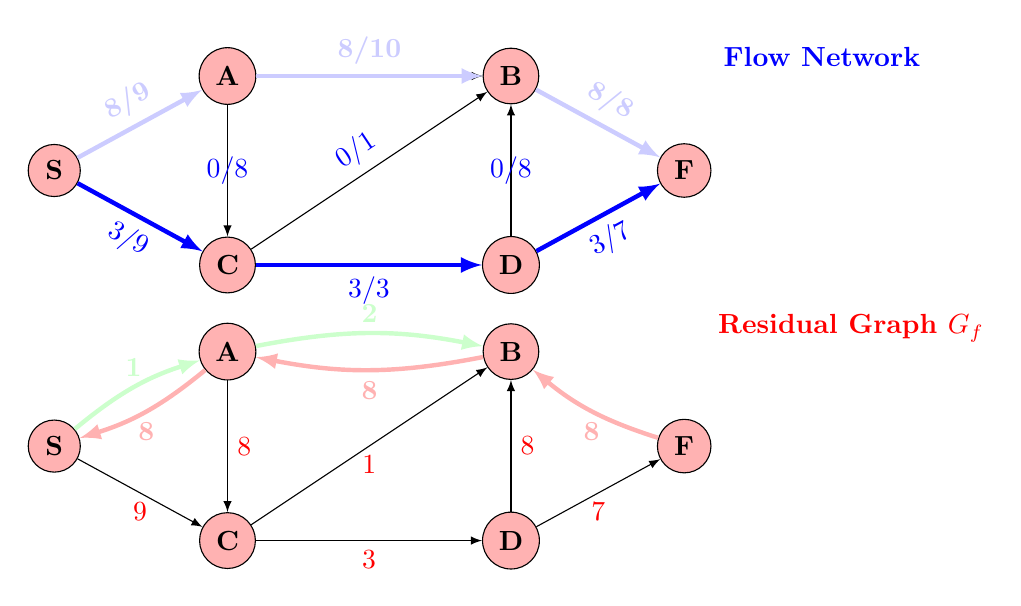
\begin{tikzpicture}
\node[draw, circle, fill=red!30, text=black, font=\bfseries, minimum size=0.5cm] (S) {S};
\node[draw, circle, fill=red!30, text=black, font=\bfseries, minimum size=0.5 cm, xshift=2.2 cm,yshift=1.2cm] (A) {A};
\node[draw, circle, fill=red!30, text=black, font=\bfseries, minimum size=0.5cm, xshift=5.8 cm,yshift=1.2cm] (B) {B};
\node[draw, circle, fill=red!30, text=black, font=\bfseries, minimum size=0.5cm, xshift=2.2 cm,yshift=-1.2cm] (C) {C};
\node[draw, circle, fill=red!30, text=black, font=\bfseries, minimum size=0.5cm, xshift=5.8 cm,yshift=-1.2cm] (D) {D};
\node[draw, circle, fill=red!30, text=black, font=\bfseries, minimum size=0.5 cm, xshift=8 cm] (F) {F};
%============
\node[draw, circle, fill=red!30, text=black, font=\bfseries, minimum size=0.5cm, below of=S, yshift=-2.5cm] (RS) {S};
\node[draw, circle, fill=red!30, text=black, font=\bfseries, minimum size=0.5 cm,below of=A, yshift=-2.5cm] (RA) {A};
\node[draw, circle, fill=red!30, text=black, font=\bfseries, minimum size=0.5cm, below of=B, yshift=-2.5cm] (RB) {B};
\node[draw, circle, fill=red!30, text=black, font=\bfseries, minimum size=0.5cm, below of=C, yshift=-2.5cm] (RC) {C};
\node[draw, circle, fill=red!30, text=black, font=\bfseries, minimum size=0.5cm, below of=D, yshift=-2.5cm] (RD) {D};
\node[draw, circle, fill=red!30, text=black, font=\bfseries, minimum size=0.5 cm,below of=F, yshift=-2.5cm] (RF) {F};
%==========

            \draw[->, blue!20, ultra thick, >=latex] (S) -- node[above, sloped, font=\bfseries\color{blue!40}] {$\textbf{8/9}$} (A);
            % \draw[->, blue, ultra thick >=latex] (S) -- node[below, sloped, font=\bfseries\color{blue}] {$0/9$} (C);
            \draw[->, blue, ultra thick, >=latex] (S) -- node[below, sloped, font=\bfseries\color{blue}] {$3/9$} (C);
            \draw[->, thin, >=latex] (A) -- node[pos = 2.5,above, sloped, font=\bfseries\color{blue}] {Flow Network} (B);
            \draw[->, blue!20, ultra thick, >=latex] (A) -- node[above, sloped, font=\bfseries\color{blue!40}] {$\textbf{8/10}$} (B);
            \draw[->, thin, >=latex] (A) -- node[
            font=\bfseries\color{blue}] {$0/8$} (C);
            \draw[->, blue!20, ultra thick, >=latex] (B) -- node[above, sloped, font=\bfseries\color{blue!40}] {$\textbf{8/8}$} (F);
            \draw[->, thin, >=latex] (C) -- node[above, sloped, font=\bfseries\color{blue}] {$0/1$} (B);
            \draw[->, blue, ultra thick, >=latex] (C) -- node[below, sloped, font=\bfseries\color{blue}] {$3/3$} (D);
            \draw[->, thin, >=latex] (D) -- node[
            font=\bfseries\color{blue}] {$0/8$} (B);
            \draw[->, blue, ultra thick, >=latex] (D) -- node[below, sloped, font=\bfseries\color{blue}] {$3/7$} (F);


            \draw[->, thin, >=latex] (RS) -- node[below, font=\bfseries\color{red}] {$9$} (RC);
            \draw[->, thin, >=latex] (RA) -- node[right,
            font=\bfseries\color{red}] {$8$} (RC);
            \draw[->, thin, >=latex] (RC) -- node[below, font=\bfseries\color{red}] {$1$} (RB);
            \draw[->, thin, >=latex] (RC) -- node[below, font=\bfseries\color{red}] {$3$} (RD);
            \draw[->, thin, >=latex] (RD) -- node[right,
            font=\bfseries\color{red}] {$8$} (RB);
            \draw[->, thin, >=latex] (RD) -- node[below, font=\bfseries\color{red}] {$7$} (RF);


             \draw[->, red!30, ultra thick, bend left=11, >=latex] (RA) to node[below, font=\bfseries\color{red}] {$\textbf{8}$} (RS);
             \draw[->, green!20, ultra thick, bend left=11, >=latex] (RS) to node[above, font=\bfseries\color{green}] {$\textbf{1}$} (RA);

             \draw[->, red!30, ultra thick, bend left=11, >=latex] (RB) to node[below, font=\bfseries\color{red}] {$\textbf{8}$} (RA);
            \node at ($(RA)!2.2!(RB)$) [above, font=\bfseries\color{red}] {Residual Graph $G_f$};
             \draw[->, green!20, ultra thick, bend left=11, >=latex] (RA) to node[above, font=\bfseries\color{green}] {$\textbf{2}$} (RB);

              \draw[->, red!30, ultra thick, bend left=11, >=latex] (RF) to node[below, font=\bfseries\color{red}] {$\textbf{8}$} (RB);
        

        
\end{tikzpicture}
\end{frame}


%===========5===============
\begin{frame}{An Example}
% \begin{columns}
%     \begin{column}{0.7\linewidth}

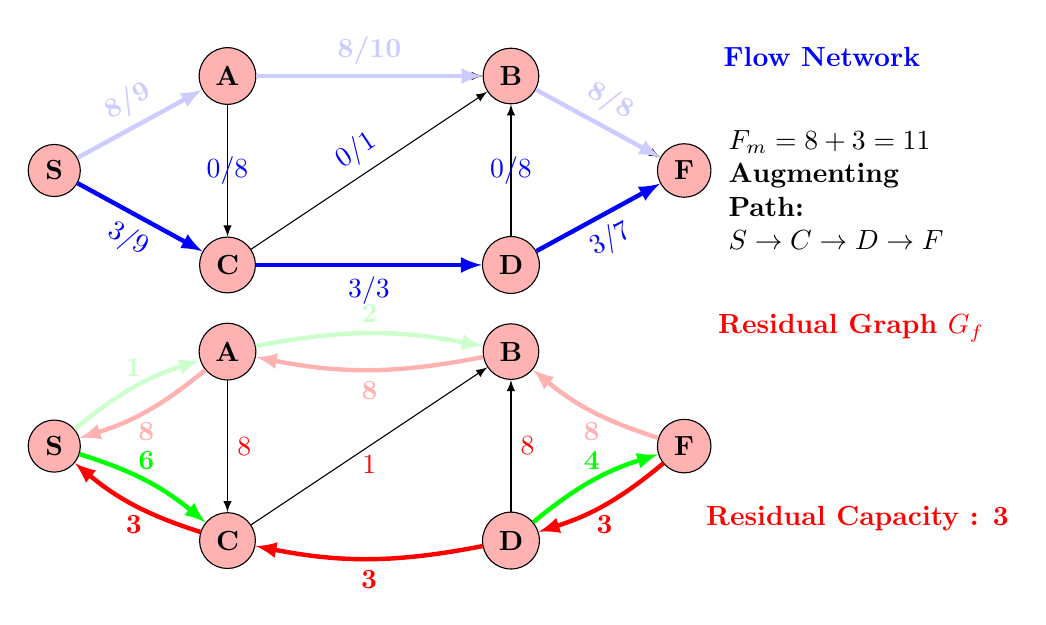
\begin{tikzpicture}
\node[draw, circle, fill=red!30, text=black, font=\bfseries, minimum size=0.5cm] (S) {S};
\node[draw, circle, fill=red!30, text=black, font=\bfseries, minimum size=0.5 cm, xshift=2.2 cm,yshift=1.2cm] (A) {A};
\node[draw, circle, fill=red!30, text=black, font=\bfseries, minimum size=0.5cm, xshift=5.8 cm,yshift=1.2cm] (B) {B};
\node[draw, circle, fill=red!30, text=black, font=\bfseries, minimum size=0.5cm, xshift=2.2 cm,yshift=-1.2cm] (C) {C};
\node[draw, circle, fill=red!30, text=black, font=\bfseries, minimum size=0.5cm, xshift=5.8 cm,yshift=-1.2cm] (D) {D};
\node[draw, circle, fill=red!30, text=black, font=\bfseries, minimum size=0.5 cm, xshift=8 cm] (F) {F};
%============
\node[draw, circle, fill=red!30, text=black, font=\bfseries, minimum size=0.5cm, below of=S, yshift=-2.5cm] (RS) {S};
\node[draw, circle, fill=red!30, text=black, font=\bfseries, minimum size=0.5 cm,below of=A, yshift=-2.5cm] (RA) {A};
\node[draw, circle, fill=red!30, text=black, font=\bfseries, minimum size=0.5cm, below of=B, yshift=-2.5cm] (RB) {B};
\node[draw, circle, fill=red!30, text=black, font=\bfseries, minimum size=0.5cm, below of=C, yshift=-2.5cm] (RC) {C};
\node[draw, circle, fill=red!30, text=black, font=\bfseries, minimum size=0.5cm, below of=D, yshift=-2.5cm] (RD) {D};
\node[draw, circle, fill=red!30, text=black, font=\bfseries, minimum size=0.5 cm,below of=F, yshift=-2.5cm] (RF) {F};
%==========

            \draw[->, blue!20, ultra thick, >=latex] (S) -- node[above, sloped, font=\bfseries\color{blue!40}] {$\textbf{8/9}$} (A);
            \draw[->, blue, ultra thick, >=latex] (S) -- node[below, sloped, font=\bfseries\color{blue}] {$3/9$} (C);
            \draw[->, thin, >=latex] (B) -- node[pos = 2.5, above, font=\bfseries\color{black}] {\parbox{3cm}{$F_m = 8 + 3 = 11$ \\ Augmenting Path: $S \rightarrow C \rightarrow D \rightarrow F$}} (F);
            
            \draw[->, thin, >=latex] (A) -- node[pos = 2.5,above, sloped, font=\bfseries\color{blue}] {Flow Network} (B);
            \draw[->, blue!20, ultra thick, >=latex] (A) -- node[above, sloped, font=\bfseries\color{blue!40}] {$\textbf{8/10}$} (B);
            \draw[->, thin, >=latex] (A) -- node[
            font=\bfseries\color{blue}] {$0/8$} (C);
            \draw[->, blue!20, ultra thick, >=latex] (B) -- node[above, sloped, font=\bfseries\color{blue!40}] {$\textbf{8/8}$} (F);
            \draw[->, thin, >=latex] (C) -- node[above, sloped, font=\bfseries\color{blue}] {$0/1$} (B);
            \draw[->, blue, ultra thick, >=latex] (C) -- node[below, sloped, font=\bfseries\color{blue}] {$3/3$} (D);
            \draw[->, thin, >=latex] (D) -- node[
            font=\bfseries\color{blue}] {$0/8$} (B);
            \draw[->, blue, ultra thick, >=latex] (D) -- node[below, sloped, font=\bfseries\color{blue}] {$3/7$} (F);
            
            % \draw[->, bend left=11]  (B) to (D);
            % \draw[->, bend left=11]  (D) to (B);

          
            \draw[->, thin, >=latex] (RA) -- node[right,
            font=\bfseries\color{red}] {$8$} (RC);
            % \draw[->, red, ultra thick, >=latex] (RB) -- node[above,  font=\bfseries\color{red}] {$\textbf{0}$} (RF);
            \draw[->, thin, >=latex] (RC) -- node[below, font=\bfseries\color{red}] {$1$} (RB);
            
            \draw[->, thin, >=latex] (RD) -- node[right,
            font=\bfseries\color{red}] {$8$} (RB);
            
             \draw[->, red!30, ultra thick, bend left=11, >=latex] (RA) to node[below, font=\bfseries\color{red}] {$\textbf{8}$} (RS);
             \draw[->, green!20, ultra thick, bend left=11, >=latex] (RS) to node[above, font=\bfseries\color{green}] {$\textbf{1}$} (RA);

             \draw[->, red!30, ultra thick, bend left=11, >=latex] (RB) to node[below, font=\bfseries\color{red}] {$\textbf{8}$} (RA);

            \node at ($(RA)!2.2!(RB)$) [above, font=\bfseries\color{red}] {Residual Graph $G_f$};
             \draw[->, green!20, ultra thick, bend left=11, >=latex] (RA) to node[above, font=\bfseries\color{green}] {$\textbf{2}$} (RB);

              \draw[->, red!30, ultra thick, bend left=11, >=latex] (RF) to node[below, font=\bfseries\color{red}] {$\textbf{8}$} (RB);
              \node at ($(RB)!2!(RF)$) [above, font=\bfseries\color{red}] {Residual Capacity : 3};
             
    

             \draw[->, red, ultra thick, bend left=11, >=latex] (RC) to node[below, font=\bfseries\color{red}] {$\textbf{3}$} (RS);
             \draw[->, green, ultra thick, bend left=11, >=latex] (RS) to node[above, font=\bfseries\color{green}] {$\textbf{6}$} (RC);

             \draw[->, red, ultra thick, bend left=11, >=latex] (RD) to node[below, font=\bfseries\color{red}] {$\textbf{3}$} (RC);

              \draw[->, red, ultra thick, bend left=11, >=latex] (RF) to node[below, font=\bfseries\color{red}] {$\textbf{3}$} (RD);
             \draw[->, green, ultra thick, bend left=11, >=latex] (RD) to node[above, font=\bfseries\color{green}] {$\textbf{4}$} (RF);

        
\end{tikzpicture}
\end{frame}

%===========6===============
%3
\begin{frame}{An Example}
% \begin{columns}
%     \begin{column}{0.7\linewidth}

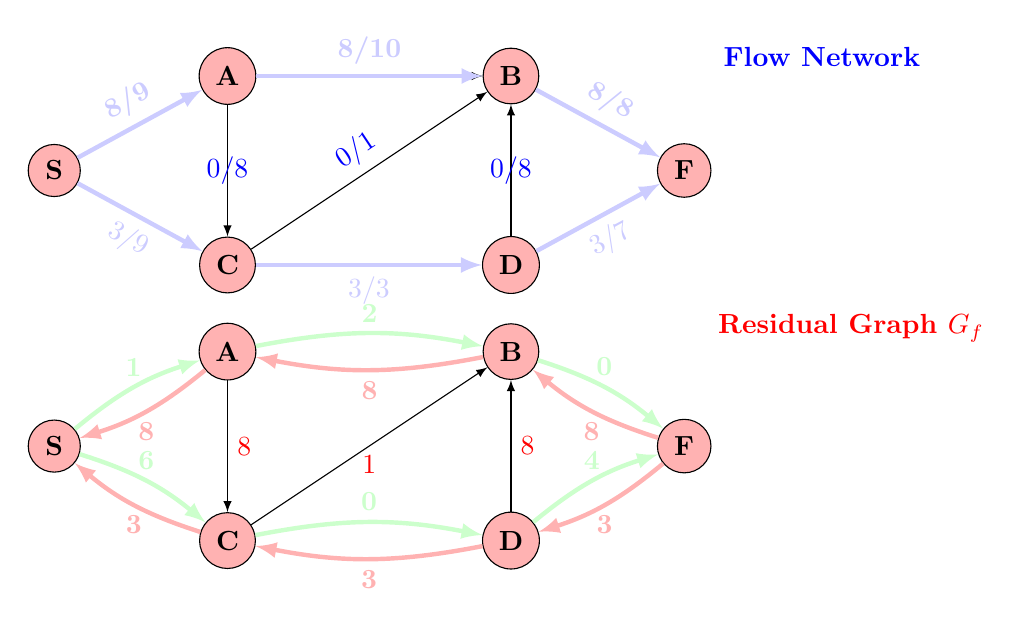
\begin{tikzpicture}
\node[draw, circle, fill=red!30, text=black, font=\bfseries, minimum size=0.5cm] (S) {S};
\node[draw, circle, fill=red!30, text=black, font=\bfseries, minimum size=0.5 cm, xshift=2.2 cm,yshift=1.2cm] (A) {A};
\node[draw, circle, fill=red!30, text=black, font=\bfseries, minimum size=0.5cm, xshift=5.8 cm,yshift=1.2cm] (B) {B};
\node[draw, circle, fill=red!30, text=black, font=\bfseries, minimum size=0.5cm, xshift=2.2 cm,yshift=-1.2cm] (C) {C};
\node[draw, circle, fill=red!30, text=black, font=\bfseries, minimum size=0.5cm, xshift=5.8 cm,yshift=-1.2cm] (D) {D};
\node[draw, circle, fill=red!30, text=black, font=\bfseries, minimum size=0.5 cm, xshift=8 cm] (F) {F};
%============
\node[draw, circle, fill=red!30, text=black, font=\bfseries, minimum size=0.5cm, below of=S, yshift=-2.5cm] (RS) {S};
\node[draw, circle, fill=red!30, text=black, font=\bfseries, minimum size=0.5 cm,below of=A, yshift=-2.5cm] (RA) {A};
\node[draw, circle, fill=red!30, text=black, font=\bfseries, minimum size=0.5cm, below of=B, yshift=-2.5cm] (RB) {B};
\node[draw, circle, fill=red!30, text=black, font=\bfseries, minimum size=0.5cm, below of=C, yshift=-2.5cm] (RC) {C};
\node[draw, circle, fill=red!30, text=black, font=\bfseries, minimum size=0.5cm, below of=D, yshift=-2.5cm] (RD) {D};
\node[draw, circle, fill=red!30, text=black, font=\bfseries, minimum size=0.5 cm,below of=F, yshift=-2.5cm] (RF) {F};
%==========

            \draw[->, blue!20, ultra thick, >=latex] (S) -- node[above, sloped, font=\bfseries\color{blue!40}] {$\textbf{8/9}$} (A);
            \draw[->, blue!20, ultra thick, >=latex] (S) -- node[below, sloped, font=\bfseries\color{blue}] {$3/9$} (C);
            \draw[->, thin, >=latex] (A) -- node[pos = 2.5,above, sloped, font=\bfseries\color{blue}] {Flow Network} (B);
            \draw[->, blue!20, ultra thick, >=latex] (A) -- node[above, sloped, font=\bfseries\color{blue!40}] {$\textbf{8/10}$} (B);
            \draw[->, thin, >=latex] (A) -- node[
            font=\bfseries\color{blue}] {$0/8$} (C);
            \draw[->, blue!20, ultra thick, >=latex] (B) -- node[above, sloped, font=\bfseries\color{blue!40}] {$\textbf{8/8}$} (F);
            \draw[->, thin, >=latex] (C) -- node[above, sloped, font=\bfseries\color{blue}] {$0/1$} (B);
            \draw[->, blue!20, ultra thick, >=latex] (C) -- node[below, sloped, font=\bfseries\color{blue}] {$3/3$} (D);
            \draw[->, thin, >=latex] (D) -- node[
            font=\bfseries\color{blue}] {$0/8$} (B);
            \draw[->, blue!20, ultra thick, >=latex] (D) -- node[below, sloped, font=\bfseries\color{blue}] {$3/7$} (F);
            
          
            \draw[->, thin, >=latex] (RA) -- node[right,
            font=\bfseries\color{red}] {$8$} (RC);
            \draw[->, thin, >=latex] (RC) -- node[below, font=\bfseries\color{red}] {$1$} (RB);
            \draw[->, thin, >=latex] (RD) -- node[right,
            font=\bfseries\color{red}] {$8$} (RB);
             \draw[->, red!30, ultra thick, bend left=11, >=latex] (RA) to node[below, font=\bfseries\color{red}] {$\textbf{8}$} (RS);
             \draw[->, green!20, ultra thick, bend left=11, >=latex] (RS) to node[above, font=\bfseries\color{green}] {$\textbf{1}$} (RA);
             \draw[->, red!30, ultra thick, bend left=11, >=latex] (RB) to node[below, font=\bfseries\color{red}] {$\textbf{8}$} (RA);
            
            \node at ($(RA)!2.2!(RB)$) [above, font=\bfseries\color{red}] {Residual Graph $G_f$};
             \draw[->, green!20, ultra thick, bend left=11, >=latex] (RA) to node[above, font=\bfseries\color{green}] {$\textbf{2}$} (RB);

              \draw[->, red!30, ultra thick, bend left=11, >=latex] (RF) to node[below, font=\bfseries\color{red}] {$\textbf{8}$} (RB);
                          
             \draw[->, green!20, ultra thick, bend left=11, >=latex] (RB) to node[above, font=\bfseries\color{green}] {$\textbf{0}$} (RF);

            

             \draw[->, red!30, ultra thick, bend left=11, >=latex] (RC) to node[below, font=\bfseries\color{red}] {$\textbf{3}$} (RS);
             \draw[->, green!20, ultra thick, bend left=11, >=latex] (RS) to node[above, font=\bfseries\color{green}] {$\textbf{6}$} (RC);

             \draw[->, red!30, ultra thick, bend left=11, >=latex] (RD) to node[below, font=\bfseries\color{red}] {$\textbf{3}$} (RC);
             \draw[->, green!20, ultra thick, bend left=11, >=latex] (RC) to node[above, font=\bfseries\color{green}] {$\textbf{0}$} (RD);

              \draw[->, red!30, ultra thick, bend left=11, >=latex] (RF) to node[below, font=\bfseries\color{red}] {$\textbf{3}$} (RD);
             \draw[->, green!20, ultra thick, bend left=11, >=latex] (RD) to node[above, font=\bfseries\color{green}] {$\textbf{4}$} (RF);
      
\end{tikzpicture}
\end{frame}

\begin{frame}[c]{An Example}
\begin{itemize}
\begin{center}
    
    \item<1-2> \textbf{\textcolor{blue!50}{\large But is there any flow remaining?}}
    \item<2-2> \textbf{\textcolor{red!50}{\Huge The Answer is no!}}
\end{center}
\end{itemize}
\end{frame}

\begin{frame}{An Example}
\begin{center}
    \color{red}{\textbf{\large THINK AGAIN! }}
    \begin{figure}
        \centering
        \includegraphics[height=5 cm, width=6cm]{imoji1.jpg}
        \label{fig:enter-label}
    \end{figure}
\end{center}
\end{frame}

\begin{frame}{An Example}
\begin{center}
    \color{red}{\textbf{\large THE ANSWER IS STILL NO !!! }}
    \begin{figure}
        \centering
        \includegraphics[height=5 cm, width=6cm]{imoji2.jpg}
        \label{fig:enter-label}
    \end{figure}
\end{center}
    
\end{frame}

\begin{frame}{An Example}

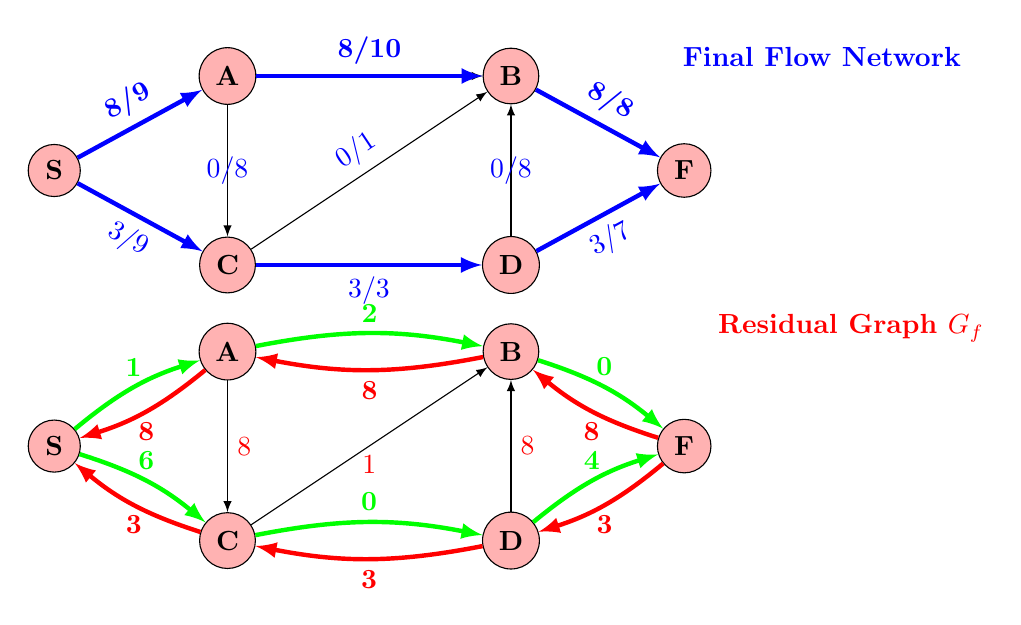
\begin{tikzpicture}
\node[draw, circle, fill=red!30, text=black, font=\bfseries, minimum size=0.5cm] (S) {S};
\node[draw, circle, fill=red!30, text=black, font=\bfseries, minimum size=0.5 cm, xshift=2.2 cm,yshift=1.2cm] (A) {A};
\node[draw, circle, fill=red!30, text=black, font=\bfseries, minimum size=0.5cm, xshift=5.8 cm,yshift=1.2cm] (B) {B};
\node[draw, circle, fill=red!30, text=black, font=\bfseries, minimum size=0.5cm, xshift=2.2 cm,yshift=-1.2cm] (C) {C};
\node[draw, circle, fill=red!30, text=black, font=\bfseries, minimum size=0.5cm, xshift=5.8 cm,yshift=-1.2cm] (D) {D};
\node[draw, circle, fill=red!30, text=black, font=\bfseries, minimum size=0.5 cm, xshift=8 cm] (F) {F};
%============
\node[draw, circle, fill=red!30, text=black, font=\bfseries, minimum size=0.5cm, below of=S, yshift=-2.5cm] (RS) {S};
\node[draw, circle, fill=red!30, text=black, font=\bfseries, minimum size=0.5 cm,below of=A, yshift=-2.5cm] (RA) {A};
\node[draw, circle, fill=red!30, text=black, font=\bfseries, minimum size=0.5cm, below of=B, yshift=-2.5cm] (RB) {B};
\node[draw, circle, fill=red!30, text=black, font=\bfseries, minimum size=0.5cm, below of=C, yshift=-2.5cm] (RC) {C};
\node[draw, circle, fill=red!30, text=black, font=\bfseries, minimum size=0.5cm, below of=D, yshift=-2.5cm] (RD) {D};
\node[draw, circle, fill=red!30, text=black, font=\bfseries, minimum size=0.5 cm,below of=F, yshift=-2.5cm] (RF) {F};
%==========

            \draw[->, blue, ultra thick, >=latex] (S) -- node[above, sloped, font=\bfseries\color{blue!40}] {$\textbf{8/9}$} (A);
            \draw[->, blue, ultra thick, >=latex] (S) -- node[below, sloped, font=\bfseries\color{blue}] {$3/9$} (C);
            \draw[->, thin, >=latex] (A) -- node[pos = 2.5,above, sloped, font=\bfseries\color{blue}] {Final Flow Network} (B);
            \draw[->, blue, ultra thick, >=latex] (A) -- node[above, sloped, font=\bfseries\color{blue!40}] {$\textbf{8/10}$} (B);
            \draw[->, thin, >=latex] (A) -- node[
            font=\bfseries\color{blue}] {$0/8$} (C);
            \draw[->, blue, ultra thick, >=latex] (B) -- node[above, sloped, font=\bfseries\color{blue!40}] {$\textbf{8/8}$} (F);
            \draw[->, thin, >=latex] (C) -- node[above, sloped, font=\bfseries\color{blue}] {$0/1$} (B);
            \draw[->, blue, ultra thick, >=latex] (C) -- node[below, sloped, font=\bfseries\color{blue}] {$3/3$} (D);
            \draw[->, thin, >=latex] (D) -- node[
            font=\bfseries\color{blue}] {$0/8$} (B);
            \draw[->, blue, ultra thick, >=latex] (D) -- node[below, sloped, font=\bfseries\color{blue}] {$3/7$} (F);
            
          
            \draw[->, thin, >=latex] (RA) -- node[right,
            font=\bfseries\color{red}] {$8$} (RC);
            \draw[->, thin, >=latex] (RC) -- node[below, font=\bfseries\color{red}] {$1$} (RB);
            \draw[->, thin, >=latex] (RD) -- node[right,
            font=\bfseries\color{red}] {$8$} (RB);
             \draw[->, red, ultra thick, bend left=11, >=latex] (RA) to node[below, font=\bfseries\color{red}] {$\textbf{8}$} (RS);
             \draw[->, green, ultra thick, bend left=11, >=latex] (RS) to node[above, font=\bfseries\color{green}] {$\textbf{1}$} (RA);
             \draw[->, red, ultra thick, bend left=11, >=latex] (RB) to node[below, font=\bfseries\color{red}] {$\textbf{8}$} (RA);
            % \draw[->, thin, >=latex] (RA) -- node[pos = 2.5,above, font=\bfseries\color{red}] {Final Residual Graph } (RB);
            \node at ($(RA)!2.2!(RB)$) [above, font=\bfseries\color{red}] {Residual Graph $G_f$};
             \draw[->, green, ultra thick, bend left=11, >=latex] (RA) to node[above, font=\bfseries\color{green}] {$\textbf{2}$} (RB);

              \draw[->, red, ultra thick, bend left=11, >=latex] (RF) to node[below, font=\bfseries\color{red}] {$\textbf{8}$} (RB);
                          
             \draw[->, green, ultra thick, bend left=11, >=latex] (RB) to node[above, font=\bfseries\color{green}] {$\textbf{0}$} (RF);



             \draw[->, red, ultra thick, bend left=11, >=latex] (RC) to node[below, font=\bfseries\color{red}] {$\textbf{3}$} (RS);
             \draw[->, green, ultra thick, bend left=11, >=latex] (RS) to node[above, font=\bfseries\color{green}] {$\textbf{6}$} (RC);

             \draw[->, red, ultra thick, bend left=11, >=latex] (RD) to node[below, font=\bfseries\color{red}] {$\textbf{3}$} (RC);
             \draw[->, green, ultra thick, bend left=11, >=latex] (RC) to node[above, font=\bfseries\color{green}] {$\textbf{0}$} (RD);

              \draw[->, red, ultra thick, bend left=11, >=latex] (RF) to node[below, font=\bfseries\color{red}] {$\textbf{3}$} (RD);
             \draw[->, green, ultra thick, bend left=11, >=latex] (RD) to node[above, font=\bfseries\color{green}] {$\textbf{4}$} (RF);
      
\end{tikzpicture}
    
\end{frame}


%%%%%%%%----------------end---------------------

\section{\textbf{Min-Cut}}

\begin{frame}{What is Cut?} 
\begin{block}{Cuts}
An s-t cut is a partition (A, B) of V with $s \in \text{A and
t} \in B$.
\end{block}
\begin{block}{}
    The capacity of a cut (A, B) is c(A,B) = $\sum_{\text{e out of A}}$ c(e)
\end{block}
\begin{block}{}
    Let f be any flow, and let (A, B) be any s-t cut.\\
    Then $\sum_\text{e out of A}$ f(e) - $\sum_\text{e into A}$ f(e) = v(f).

\end{block}
\end{frame}

\begin{frame}{Max Flow - Min Cut}
\begin{block}{Min-Cut}
Min-cut is the one with the minimum total capacity. It has the smallest sum of capacities among all cuts that separate the source and sink nodes.\\
The \textcolor{blue}{value of the minimum cut is equal to the maximum flow in the network, which is a fundamental property exploited by the Ford-Fulkerson algorithm} for finding the maximum flow.
\end{block}
\end{frame}

\begin{frame}{Maxflow-Mincut Theorem}
\begin{block}{Conditions}
If f is a flow in a flow network G=(V,E), with source s and sink t, then the following conditions are equivalent:\\
\begin{itemize}
    \renewcommand{\labelitemi}{$\Rightarrow$}
    \item f is a maximum flow in G.
    \item The residual network $G_f$ contains no augmented paths.
    \item $|f| = c(S,T)$ for some cut (S,T) (a min-cut).
\end{itemize}
It is a flow since there is no augmented paths It is maximum since the sink is not reachable from the source
\end{block} 
\end{frame}

\begin{frame}{Min-Cut Example}
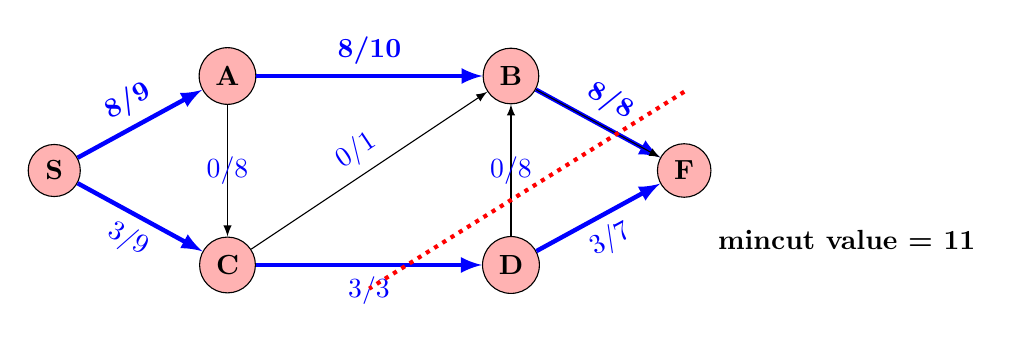
\begin{tikzpicture}
\node[draw, circle, fill=red!30, text=black, font=\bfseries, minimum size=0.5cm] (S) {S};
\node[draw, circle, fill=red!30, text=black, font=\bfseries, minimum size=0.5 cm, xshift=2.2 cm,yshift=1.2cm] (A) {A};
\node[draw, circle, fill=red!30, text=black, font=\bfseries, minimum size=0.5cm, xshift=5.8 cm,yshift=1.2cm] (B) {B};
\node[draw, circle, fill=red!30, text=black, font=\bfseries, minimum size=0.5cm, xshift=2.2 cm,yshift=-1.2cm] (C) {C};
\node[draw, circle, fill=red!30, text=black, font=\bfseries, minimum size=0.5cm, xshift=5.8 cm,yshift=-1.2cm] (D) {D};
\node[draw, circle, fill=red!30, text=black, font=\bfseries, minimum size=0.5 cm, xshift=8 cm] (F) {F};

             \draw[->, blue, ultra thick, >=latex] (S) -- node[above, sloped, font=\bfseries\color{blue!40}] {$\textbf{8/9}$} (A);
            \draw[->, blue, ultra thick, >=latex] (S) -- node[below, sloped, font=\bfseries\color{blue}] {$3/9$} (C);
            % \draw[->, thin, >=latex] (A) -- node[pos = 2.5,above, sloped, font=\bfseries\color{blue}] {Final Flow Network} (B);
            \draw[->, blue, ultra thick, >=latex] (A) -- node[above, sloped, font=\bfseries\color{blue!40}] {$\textbf{8/10}$} (B);
            \draw[->, thin, >=latex] (A) -- node[
            font=\bfseries\color{blue}] {$0/8$} (C);
            \draw[->, blue, ultra thick, >=latex] (B) -- node[above, sloped, font=\bfseries\color{blue!40}] {$\textbf{8/8}$} (F);
            \draw[->, thin, >=latex] (C) -- node[above, sloped, font=\bfseries\color{blue}] {$0/1$} (B);
            \draw[->, blue, ultra thick, >=latex] (C) -- node[below, sloped, font=\bfseries\color{blue}] {$3/3$} (D);
            \draw[->, thin, >=latex] (D) -- node[
            font=\bfseries\color{blue}] {$0/8$} (B);
            \draw[->, blue, ultra thick, >=latex] (D) -- node[below, sloped, font=\bfseries\color{blue}] {$3/7$} (F);

            \draw[->, thin, >=latex] (B) -- node[pos = 2.5, above, font=\bfseries\color{black}] {mincut value = 11} (F);

            
            \draw[dotted, line width=1.5pt, red] (8, 1) -- (4, -1.5);
\end{tikzpicture}
\end{frame}



\begin{frame}{}
    \begin{columns}
        \column{0.35\textwidth}
        \centering
        \includegraphics[scale=0.75]{images/see.png}
        
        \column{0.65\textwidth}
        \centering
        {\Huge \textcolor{red}{See!!}}\\
        \vspace{0.75cm}
        \begin{block}
             
        \textcolor{blue}{Mincut Value v(f) $\Leftrightarrow$ Maxflow $|M_f| = 11$}
        \end{block}
    \end{columns}
\end{frame}



\section{\textbf{Running Time Complexity}}
\begin{frame}{Running Time?}
\begin {center} 
\begin {minipage} {0.8\textwidth}
\begin{block}{}
 The running time depends on\\
         \begin{itemize}
             \item[\ding{51}]Number of augmenting paths needed to find a maxflow
             \item[\ding{51}] Time needed to find each augmenting path
         \end{itemize}
         \end{block}
\begin{block}{Running Time}
         Find a residual path $\rightarrow$  O(m+n)\\
         Compute bottleneck capacity $\rightarrow$  O(m)\\
         Update flow  $\rightarrow$  O(m)\\
         Update residual graph $\rightarrow$  O(m)\\
         \textcolor{blue}{Total running time $\rightarrow$ O(C(m+n))}
\end{block} 
\end{minipage}
\end{center}
\end{frame}

\begin{frame}{Running Time?}
\begin {center} 
\begin {minipage} {0.9\textwidth}
\begin{block}{Analysis}
\begin{cases}
    \text{\textbf{for} each edge \text{(u,v)} } \in E[G]  \\
    &\quad \textbf{do } \text{f[u,v]} \leftarrow 0\\
    &\quad \quad \text{ f[u,v]} \leftarrow 0\\
\end{cases}

\textbf{while} there exits a path p from s to t in the residual network G_f\\
\begin{cases}
&\quad \quad \textbf{do } c_f\text{(p)} \leftarrow min\ c_f \{\text{(u,v):(u,v)}\text{is in p} \}\\
&\quad \quad \quad  \text{\textbf{for} each edge \text{(u,v)} } \text{in p}\\
&\quad \quad \quad \quad \textbf{do } \text{f[u,v]} \leftarrow \text{f[u,v]} + c_f\text{(p)}\\
&\quad \quad \quad \quad \quad \text{  f[u,v]} \leftarrow \text{-f[u,v]}
\end{cases}\\
\end{block}
\textcolor{red}{O(E) for both cases 'indicated by \{'}
\end{minipage}
\end{center}
\end{frame}

\begin{frame}{Running Time?}
\begin {center} 
\begin {minipage} {0.9\textwidth}  
\begin{block}{Analysis}
    \begin{itemize}
        \item[$\circ$] If capacities are all integers, then each augmenting path raises $|f|$ by $\geq 1$.
        \item[$\circ$] If maxflow is $f^{\star}$, then need $\leq |f^{\star}|$ iterations.
        \item[$\circ$] So the time complexity is $O(E|f^{\star}|)$.
        \item[$\circ$] This running time is not polynomial in input size. It depends on $f^{\star}$, which is not a function of $|V|$ or $|E|$.
        \item[$\circ$] If capacities are rational, you can scale them to integers.
        \item[$\circ$] If capacities are irrational, the Ford-Fulkerson algorithm might never terminate!
    \end{itemize}
\end{block}
\end{minipage}
\end{center}
\end{frame}

\begin{frame}
    \begin{center}
       \includegraphics{images/thanks.png}
    \end{center}
\end{frame}

\begin{frame}
    \begin{center}
       \includegraphics{images/question.png}
    \end{center}
\end{frame}




\end{document}
